%%%%%%%%%%%%%%%%%%%%%%%%%%%%%%%%%%%%%%%%%%%%%%%%%%%%%%%%%%%%%%%%%%%%%%
% Lớp 11 | Quan hệ vuông góc trong không gian | Hình lăng trụ đứng. Hình chóp đều. Thể tích
% Dạng 1H8?7-1: Câu hỏi lý thuyết, công thức
% Số câu: 26  (sinh tự động bởi tach_cau.py; từ nay thầy sửa trực tiếp file này)
%%%%%%%%%%%%%%%%%%%%%%%%%%%%%%%%%%%%%%%%%%%%%%%%%%%%%%%%%%%%%%%%%%%%%%

%%%%%%%%%%%%%%%% TRẮC NGHIỆM 4 PHƯƠNG ÁN %%%%%%%%%%%%%%%%

% nguồn: Ok_Toan11_TracNghiem_Lan2
\begin{ex}%[1H8N7-1]%[ma:5deba477]
	Cho khối chóp có diện tích đáy $S=5a^2$ và  chiều cao $h=a$. Thể tích của khối chóp đã cho bằng
	 \choice
		 {$\dfrac{5}{6}{a^3}$}
		 {$\dfrac{5}{2}{a^3}$}
		 {$ 5a^3$}
		{\True  $\dfrac{5}{3}{a^3}$}
	 \loigiai{
	Thể tích của khối chóp đã cho bằng $ V=\dfrac{1}{3}\cdot S\cdot  h=\dfrac{1}{3}\cdot5a^2\cdot a=\dfrac{5}{3}{a^3}$.}
\end{ex}

% nguồn: Ok_Toan11_TracNghiem_Lan2
\begin{ex}%[1H8N7-1]%[ma:ea41fcc4]
	Cho khối lăng  trụ có diện tích đáy $B=3$ và chiều cao $h=2$. Thể tích của khối lăng trụ đã cho bằng
	\choice 
		{$1$} 
		 {$3$}
		{$2$} 
		{\True  $6$}
	 \loigiai{
		Thể tích khối lăng trụ là $V = B \cdot h = 3 \cdot  2 = 6$.
	 }
\end{ex}

% nguồn: Ok_Toan11_TracNghiem_Lan2
\begin{ex}%[1H8N7-1]%[ma:27b3c9c7]
	Thể tích của khối lập phương cạnh $2a$ bằng 
	\choice 
		 {$a^3$}
		{$2a^3$} 
		{\True  $8a^3$}
		 {$4a^3$}
	 \loigiai{
	Ta có  $V=(2a)^3=8a^3$.}
\end{ex}

% nguồn: Ok_Toan11_TracNghiem_Lan2
\begin{ex}%[1H8N7-1]%[ma:a42934b6]
	Thể tích của khối chóp có  diện tích đáy bằng $\dfrac{\sqrt{3}}{2}$ và chiều cao bằng $\dfrac{2\sqrt{3}}{3}$ là
	 \choice
		{$\dfrac{\sqrt{6}}{6}$} 
		 {\True $\dfrac{1}{3}$}
		{$\dfrac{\sqrt{2}}{3}$} 
		 {$1$}
	\loigiai{ 
		Thể tích khối chóp được tính bằng công thức $V = \dfrac{1}{3}  \cdot B \cdot h$.\\
		Trong đó $B$ là diện tích  đáy và $h$ là chiều cao.\\
		Khi đó, ta  có
		$$V = \dfrac{1}{3} \cdot \dfrac{\sqrt{3}}{2} \cdot  \dfrac{2\sqrt{3}}{3} = \dfrac{1}{3}.$$
	 }
\end{ex}

% nguồn: Ok_Toan11_TracNghiem_Lan2
\begin{ex}%[1H8N7-1]%[ma:5b604d51]
	Cho khối chóp có diện tích đáy $B=6$ và chiều cao $h=2$. Thể tích của khối chóp đã cho  bằng:
	\choice 
		 {$6$}
		 {$3$}
		{\True $4$} 
		{$12$} 
	\loigiai{ 
	Thể tích của  khối chóp $V=\dfrac{1}{3}Bh=4$.}
\end{ex}

% nguồn: Ok_Toan11_TracNghiem_Lan2
\begin{ex}%[1H8N7-1]%[ma:64fcde9a]
	Cho khối lăng trụ có diện tích đáy $B=4a^2$ và chiều cao $h=a$. Thể tích của khối lăng trụ đã  cho bằng
	 \choice
		 {$\dfrac{2}{3}a^3$}
		{\True  $4a^3$}
		{$\dfrac{4}{3}a^3$} 
		{$2a^3$} 
	 \loigiai{
	Thể tích của  khối lăng trụ đã cho bằng $V=B\cdot h=4a^2\cdot a=4a^3$.}
\end{ex}

% nguồn: Ok_Toan11_TracNghiem_Lan2
\begin{ex}%[1H8N7-1]%[ma:2264fa33]
	Cho khối chóp  có diện tích đáy $B=3$ và chiều cao $h=2$. Thể tích khối chóp đã cho bằng
	\choice 
		 {$6$}
		 {$12$}
		{\True  $2$}
		 {$3$}
	 \loigiai{
	Thể tích khối chóp đã  cho là $V=\dfrac{1}{3}Bh=\dfrac{1}{3}\cdot 3\cdot 2=2$.}
\end{ex}

% nguồn: Ok_Toan11_TracNghiem_Lan2
\begin{ex}%[1H8N7-1]%[ma:2f9e1bd9]
	Thể tích của khối  lập phương cạnh $4a$ bằng
	 \choice
		 {\True $64a^3$}
		{$32a^3$} 
		{$16a^3$} 
		{$8a^3$} 
	 \loigiai{
	Thể tích của khối lập phương cạnh $4a$  là $V=(4a)^3=64a^3$.}
\end{ex}

% nguồn: Ok_Toan11_TracNghiem_Lan2
\begin{ex}%[1H8N7-1]%[ma:f45e434c]
	Cho khối chóp có diện tích đáy $S=7a^2$  và chiều cao $h=a$. Thể tích của khối chóp đã cho bằng
	\choice 
		 {$\dfrac{7}{6}{a^3}$}
		{$\dfrac{7}{2}{a^3}$} 
		{\True $\dfrac{7}{3}{a^3}$} 
		 {$ 7a^3$}
	\loigiai{ 
	Thể tích khối chóp $V=\dfrac{1}{3}\cdot S\cdot h=\dfrac{1}{3}\cdot7a^2\cdot a=\dfrac{7}{3}{a^3}$.} 
\end{ex}

% nguồn: Ok_Toan11_TracNghiem_Lan2
\begin{ex}%[1H8N7-1]%[ma:c32f9a99]
	 Cho khối chóp có diện tích đáy $B=3$ và chiều cao $h=4$. Thể tích của khối chóp đã cho bằng
	 \choice
		{$6$} 
		{$12$} 
		 {$36$}
		{\True $4$} 
	\loigiai{ 
	Ta có công thức thể tích khối chóp $V=\dfrac{1}{3}\cdot B\cdot h=\dfrac{1}{3}\cdot  3\cdot 4=4$.}
\end{ex}

% nguồn: Ok_Toan11_TracNghiem_Lan2
\begin{ex}%[1H8N7-1]%[ma:86d7ce6c]
	Thể tích  của khối lập phương cạnh $5a$ bằng
	\choice 
		{$5a^3$} 
		 {$a^3$}
		{\True $125a^3$} 
		 {$25a^3$}
	 \loigiai{
		Thể tích của khối lập phương  cạnh bằng $5a$ là\\
	$V=(5a)^3=125a^3$.} 
\end{ex}

% nguồn: Ok_Toan11_TracNghiem_Lan2
\begin{ex}%[1H8N7-1]%[ma:4026ff76]
	Thể tích khối hộp chữ nhật có ba kích thước $2$,  $3$, $7$ bằng
	 \choice
		 {$14$}
		{\True  $42$}
		 {$126$}
		 {$12$}
	\loigiai{ 
	Thể tích khối hộp có ba  kích thước $2$, $3$, $7$ bằng $V=abc=2\cdot 3\cdot 7=42$.}
\end{ex}

% nguồn: Ok_Toan11_TracNghiem_Lan2
\begin{ex}%[1H8N7-1]%[ma:5c6314d3]
	Cho khối lăng trụ có diện tích đáy là $3a^2$ và chiều cao $2a$. Thể tích khối lăng trụ đã cho bằng 
	 \choice
		{$a^3$} 
		{\True $6a^3$} 
		 {$3a^3$}
		 {$2a^3$}
	 \loigiai{
	Ta có $V=B\cdot h=3a^2\cdot 2a=6a^3$.} 
\end{ex}

% nguồn: Ok_Toan11_TracNghiem_Lan2
\begin{ex}%[1H8N7-1]%[ma:90234846]
	Cho khối chóp có diện tích đáy $S=8a^2$ và chiều cao $h=a$. Thể tích của khối chóp đã  cho bằng
	 \choice
		{$8  a^3$}
		{$\dfrac{4}{3}a^3$} 
		{$4 a^3$} 
		{\True $\dfrac{8}{3}a^3$} 
	\loigiai{ 
	Thể tích của khối chóp có diện tích đáy $S=8a^2$ và chiều cao $h=a$  là $$V=\dfrac{1}{3}\cdot S\cdot h=\dfrac{1}{3}\cdot8a^2\cdot a=\dfrac{8}{3}{a^3}.$$}
\end{ex}

% nguồn: Ok_Toan11_TracNghiem_Lan2
\begin{ex}%[1H8N7-1]%[ma:6d6b751d]
	Một khối chóp có diện tích đáy bằng $6$ và chiều cao bằng $5$. Thể tích của khối  chóp đã cho bằng
	 \choice
		{\True  $10$}
		{$30$} 
		 {$90$}
		{$15$} 
	\loigiai{Ta  có
	$$V=\dfrac{1}{3}\cdot  S\cdot h=\dfrac{1}{3}\cdot6\cdot5=10.$$}
\end{ex}

% nguồn: Ok_Toan11_TracNghiem_Lan2
\begin{ex}%[1H8N7-1]%[ma:10fed8ad]
	Cho khối chóp có diện tích đáy $B=6a^2$  và chiều cao $h=2a$. Thể tích khối chóp đã cho bằng:
	 \choice
		 {$2a^3$}
		{\True  $4a^3$}
		 {$6a^3$}
		{$12a^3$} 
	 \loigiai{
	Thể tích  khối chóp đã cho là $V=\dfrac{1}{3}B\cdot h=\dfrac{1}{3}6a^2\cdot 2a=4a^3$.}
\end{ex}

% nguồn: Ok_Toan11_TracNghiem_Lan2
\begin{ex}%[1H8N7-1]%[ma:aed6f1f6]
	Thể  tích khối lập phương có độ dài cạnh $3a$ bằng
	 \choice
		{\True  $27a^3$}
		{$3a^3$} 
		{$9a^3$} 
		 {$a^3$}
	\loigiai{ 
	Thể tích khối lập phương là $(3a)^3=27a^3$.} 
\end{ex}

% nguồn: Ok_Toan11_TracNghiem_Lan2
\begin{ex}%[1H8N7-1]%[ma:a771ceaf]
	 Cho khối lập phương có cạnh bằng $6$. Thể tích của khối lập phương đã cho bằng
	\choice 
		{\True $216$} 
		 {$18$}
		 {$36$}
		 {$72$}
	\loigiai{ 
	Thể tích khối lập phương có cạnh bằng $6$ là $V=6^3=216$.} 
\end{ex}

% nguồn: Ok_Toan11_TracNghiem_Lan2
\begin{ex}%[1H8N7-1]%[ma:cda4eba7]
	Cho khối trụ có diện tích đáy $B=2a^2$ và chiều cao $h=a$. Thể tích của khối trụ  đã cho bằng
	\choice 
		{$\dfrac{2}{3}a^3$} 
		 {$a^3$}
		{$\dfrac{1}{3}a^3$} 
		{\True  $2a^3$}
	 \loigiai{
	Thể tích khối trụ là $V=B\cdot h=2a^2\cdot  a=2a^3$.}
\end{ex}

% nguồn: Ok_Toan11_TracNghiem_Lan2
\begin{ex}%[1H8N7-1]%[ma:abcf4584]
	Thể tích khối  lăng trụ có diện tích đáy $B$ và có chiều cao $h$ là
	 \choice
		{\True  $Bh$}
		 {$\dfrac{4}{3}Bh$}
		 {$\dfrac{1}{3}Bh$}
		{$3Bh$} 
	 \loigiai{
	 Thể tích khối lăng trụ có diện tích đáy $B$ và có chiều cao $h$ là $V=B\cdot h$.}
\end{ex}

% nguồn: Ok_TracNghiemLop11_Lan1
\begin{ex}%[1H8N7-1]%[ma:1009b228]
	Cho hình chóp tứ giác đều $S.ABCD$ có $ O$ là giao điểm  $ AC$ và $BD$. Khẳng định nào sau đây \textbf{sai}?
	\choice 
		{\True Các mặt bên là các tam giác  đều}
		{$SA=SB=SC=SD$} 
		{$ABCD$  là hình vuông}
		{$SO \perp(ABCD)$} 
	\loigiai{ 
		Hình chóp tứ giác  đều $S.ABCD$ các cạnh bên bằng nhau nên mệnh đề \lq\lq Các mặt bên là các tam giác đều\rq\rq.
	} 
\end{ex}

% nguồn: Ok_TracNghiemLop11_Lan1
\begin{ex}%[1H8N7-1]%[ma:feb19f16]
	Cho khối chóp có diện tích đáy $B$ và chiều cao $h$. Thể tích $V$ của khối chóp đã cho được  tính theo công thức nào dưới đây?
	 \choice
		{\True $V=\dfrac{1}{3}Bh$} 
		 {$V=Bh$}
		 {$V=\dfrac{4}{3}Bh$}
		 {$V=\dfrac{1}{2}Bh$}
	 \loigiai{
	Công thức thể tích khối  chóp là $V=\dfrac{1}{3}Bh$.}
\end{ex}

% nguồn: Ok_TracNghiemLop11_Lan1
\begin{ex}%[1H8N7-1]%[ma:8d99d897]
	Khẳng định nào  sau đây đúng?
	\choice 
		{Hình lăng trụ có đáy là  một đa giác đều là hình lăng trụ đều}
		{Hình lăng trụ đứng là hình lăng trụ  đều}
		{\True Hình lăng trụ đứng có đáy là một đa giác  đều là hình lăng trụ đều}
		{Hình lăng  trụ tứ giác đều là hình lập phương}
	\loigiai{ 
		Theo định  nghĩa ta có \lq\lq Hình lăng trụ đứng có đáy là một đa giác đều là hình lăng trụ đều\rq\rq.
	 }
\end{ex}

% nguồn: Ok_TracNghiemLop11_Lan1
\begin{ex}%[1H8N7-1]%[ma:a09af2b5]
	 Trong các khẳng định sau về hình lăng trụ đều, khẳng định nào là \textbf{sai}?
	\choice 
		{\True Các  mặt bên là những hình vuông}
		{Các cạnh bên vuông góc với  mặt đáy}
		{Các mặt bên là những hình chữ nhật nằm trong  mặt phẳng vuông góc với mặt đáy}
		{Đáy  là đa giác đều}
	 \loigiai{
	Hình lăng trụ đều là một loại hình lăng trụ  đứng, có đáy là một đa giác đều.}
\end{ex}

% nguồn: Ok_TracNghiemLop11_Lan1
\begin{ex}%[1H8H7-1]%[ma:d48c8f51]
	Cho hình lập phương $ABCD.A'B'C'D'$. Tính góc giữa hai đường thẳng $AC$  và $A'B$.
	\choice 
		 {\True $60^\circ$}
		 {$45^\circ$}
		 {$75^\circ$}
		 {$90^\circ$}
	 \loigiai{
	\immini{ 
		Do $A'BCD'$ là hình bình hành nên $A'B\parallel D'C$. Suy ra góc  giữa hai đường thẳng $AC$ và $A'B$ bằng góc giữa hai đường thẳng $AC$ và $D'C$ và đó chính là góc $\widehat{ACD'}=60^\circ$ (do $\triangle ACD'$ đều).
		} 
		 {
		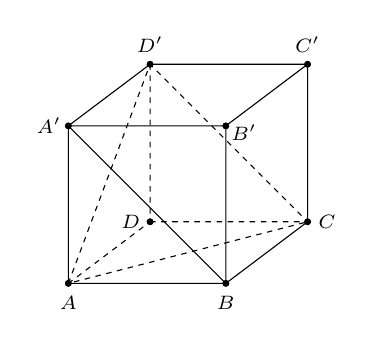
\begin{tikzpicture}[declare function={r=2;}]
				\path (0:0) coordinate (A) 
					(0:r) coordinate  (B)
					++(37:{0.65*r}) coordinate  (C)
					++(180:r)  coordinate (D)
				\foreach \x in  {A,B,C,D}{(\x)++(90:r) coordinate (\x')};
				\draw[dash pattern=on 2pt off  2 pt] (D')--(D)--(A)
					 (D)--(C)--(D')--(A)--(C);
				\draw  (A)--(B)--(C)
					(A)--(A') 
					 (B)--(B')
					 (C)--(C')
					(A')--(B')--(C')--(D')--cycle (A')--(B); 
				\foreach \x  in {A,B,C,D,A',B',C',D'}
				\draw[fill]  (\x) circle (1pt);
				 \foreach \t/\g in {A/-90,B/-90,C/0,D/180,A'/180,B'/-20,C'/90,D'/90}{
					\draw[fill]  (\t) circle (1pt) node[shift={(\g:7pt)},font=\scriptsize]{$ \t $};
				} 
			\end{tikzpicture}
		 }
	} 
\end{ex}

% nguồn: Ok_TracNghiemLop11_Lan1
\begin{ex}%[1H8Y7-1]%[ma:38619787]
	Cho hình chóp tam giác đều $S.ABC$. Khẳng định nào sau đây là  \textbf{sai} về hình chóp đã cho?
	\choice 
		{Tam giác  $ABC$ là tam giác đều}
		{Các cạnh bên hợp với đáy các góc bằng  nhau}
		{\True Các mặt bên là các tam giác  đều}
		 {Các mặt bên hợp với đáy các góc bằng nhau}
	 \loigiai{
		Hình chóp tam giác đều có các mặt bên là  các tam giác cân.
	 }
\end{ex}
